%%%%%%%%%%%%%%%%%%%%%%%%%%%%%%%%%%%%%%%%%%%%%%%%%%%%%%%%%%%%%%%%%%%%%%%%%%%
%%  introduction_v10.tex  –  Введение (ненумерованная глава)
%%  v10 – Обновлено в соответствии с финальными слайдами презентации.
%%       Новое название диссертации: «Разработка состязательных устойчивых
%%       моделей в гибридных системах обнаружения и предотвращения вторжений»
%%       Научная новизна переписана как концепции/теории (не модели).
%%       Объект/предмет обновлены для гибридных IDPS.
%%       Цитирование начинается с [1].
%%%%%%%%%%%%%%%%%%%%%%%%%%%%%%%%%%%%%%%%%%%%%%%%%%%%%%%%%%%%%%%%%%%%%%%%%%%

\chapter*{ВВЕДЕНИЕ}
\addcontentsline{toc}{chapter}{Введение}
\markboth{ВВЕДЕНИЕ}{ВВЕДЕНИЕ}

%%---------------------------------------------------------------------
\section*{Актуальность темы исследования}
%%---------------------------------------------------------------------

\emph{Гибридные системы обнаружения и предотвращения вторжений}
(далее~--- гибридная СОПВ) являются основным защитным контуром
информационных систем в критически важных областях: сетевом
трафике, БПЛА, банковско-финансовой и медицинской инфраструктуре,
промышленном IoT и АСУ~ТП, автономных транспортных средствах,
облачных и SaaS-инфраструктурах. Они объединяют сигнатурные,
аномалийные, статистические и обучаемые компоненты со средствами
реагирования и интеграцией с SIEM/SOAR. Однако робастность
существующих IDPS~--- способность сохранять качество обнаружения
при состязательных воздействиях, в распределённых и нестационарных
условиях~--- отстаёт от точности на
25--65~процентных пунктов~\cite{Zuegner2018,Bojchevski2019,Dai2018,Goodfellow2014gan,Szegedy2014},
что делает \emph{актуальной} разработку моделей и алгоритмов
повышения их робастности и эффективности.
Работа посвящена \emph{разработке состязательных устойчивых
ИИ-моделей в гибридных СОПВ для сетевой безопасности}, на
инстанции защиты сетевого трафика (NIDPS) с переносом в сектор
защиты БПЛА; все шесть сквозных свойств P1--P6 сохраняются как
обязательные требования к AI-моделям.

Под \emph{гибридной системой обнаружения и предотвращения вторжений}
(гибридная СОПВ) понимается класс \emph{ИИ/МО-усиленных} защитных
контуров, объединяющих три канонических канала детектирования~---
\emph{сигнатурный}, \emph{аномалийный} и \emph{протокольный}~---
усиленных моделями ИИ/МО на каждом канале. В отличие от
конвенциональных IDPS (Snort\,3, Suricata, Zeek, Cisco~IPS,
Palo~Alto~Threat~Prevention, McAfee~NSP), реализующих эти каналы
без обучаемого слоя, гибридная СОПВ преодолевает три систематические
неэффективности: \emph{(а)} слепоту сигнатурного канала к атакам
нулевого дня (задержка 30--90~дней до включения
сигнатуры~\cite{Sachkov2022threat}); \emph{(б)} высокий уровень ложных
срабатываний аномалийного канала ($10^{-2}$--$10^{-1}$ на нормальный
поток, вызывающий alert fatigue~\cite{FerragPoisoning2023});
\emph{(в)} ограниченность семантического контекста протокольного
канала с масштабированием $\mathcal{O}(P\cdot S)$ по протоколам~$P$
и состояниям~$S$. Модели~М1--М7 из Главы~\ref{ch:methods}
закрывают эти неэффективности: сертифицированную робастность
обеспечивают М1, М4, М7 (П1 из~\S\ref{subsec:six_properties});
калиброванную неопределённость~--- М5--М6 (П5); адаптацию к новым
протоколам~--- М3 и CyberSecLLM (П6). Концептуальная схема
приведена на рис.~\ref{fig:hybrid_idps_overview}.

\begin{figure}[htbp]
\centering
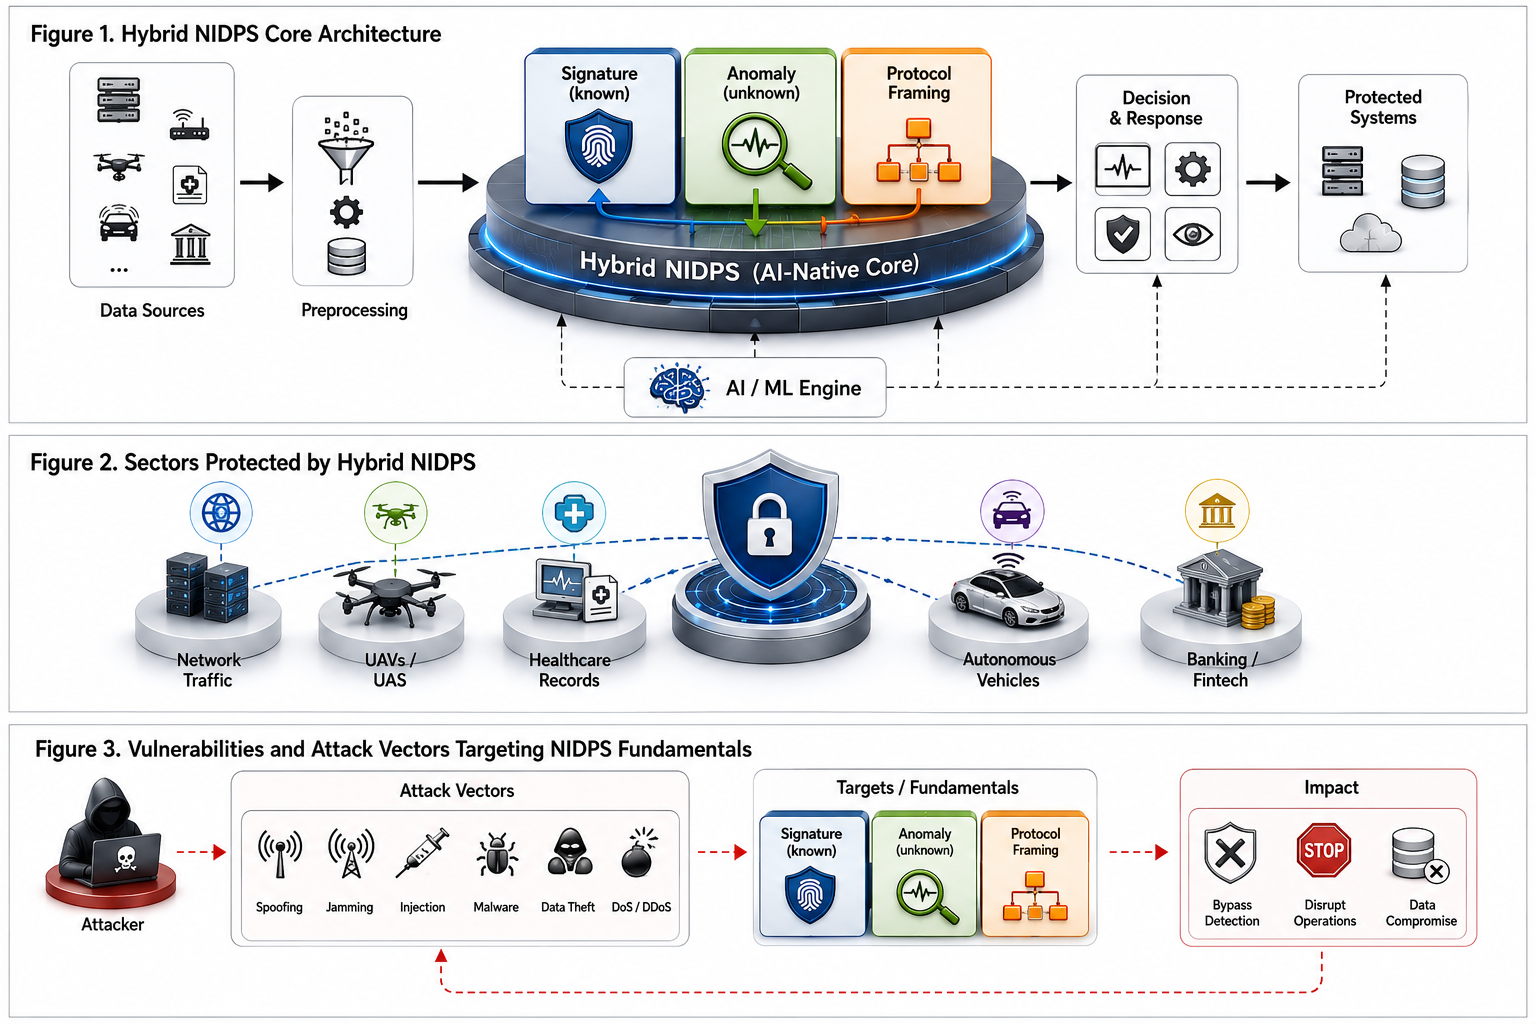
\includegraphics[width=0.96\textwidth]{figures/fig_nidps_v2.png}
\caption{Концептуальная схема гибридной СОПВ в трёх аспектах.
\textbf{Сверху}~--- ядро архитектуры (Hybrid~NIDPS AI-Native Core)
с трёхканальным детектированием (сигнатурный, аномалийный,
протокольный), AI/ML-движком в качестве усиливающего слоя,
блоком принятия решений и реагирования и защищаемыми системами.
\textbf{В центре}~--- предметные области применения системы:
сетевой трафик, БПЛА, медицинские записи, автономные транспортные
средства, банковско-финансовая инфраструктура.
\textbf{Снизу}~--- поверхность атак на канонические компоненты:
атакующий → векторы атак (спуфинг, джемминг, инъекция, malware,
утечка данных, DoS/DDoS) → целевые компоненты (signature,
anomaly, protocol framing) → последствия (обход обнаружения,
нарушение работы, компрометация данных).}
\label{fig:hybrid_idps_overview}
\end{figure}

Анализ существующих гибридных СОПВ в Главе~\ref{ch:literature}
выявляет четыре взаимосвязанные проблемы:
\emph{(1)} уязвимость обучаемых детекторов к малым возмущениям
входных данных и графовых связей; \emph{(2)} неспособность
обрабатывать новые паттерны угроз без переобучения;
\emph{(3)} чрезмерная вычислительная стоимость, исключающая работу
в реальном времени; \emph{(4)} отсутствие формальных гарантий
приватности при федеративном обучении. Эти проблемы взаимосвязаны
архитектурным корнем~--- использованием моделей с двойственным
входом (графовые нейронные сети, модели пространства состояний,
стохастические дифференциальные модели, байесовские сети,
теоретико-игровые алгоритмы).

Графовые нейронные сети~(ГНС)~\cite{Kipf2017,Velickovic2018,Hamilton2017,Wu2020gnn_survey,Luo2021}~---
одна из наиболее распространённых ветвей моделей в гибридная СОПВ,
а проблемы~(1)--(4) наиболее наглядно проявляются именно в моделях
с двойственным входом. ГНС-модель одновременно получает числовые
\emph{данные} ($\mathbf{X}\in\mathbb{R}^{n\times d}$, матрица
признаков) и реляционную \emph{структуру} ($\mathbf{A}$, матрица
смежности), формируя выход через итеративную агрегацию окрестностей.
Возмущение любого из входов может нарушить предсказания. Эта
двойственная природа входов отличает ГНС от обычных нейронных
сетей и образует источник проблем робастности, решаемых в работе
для нескольких ветвей моделей одновременно.

\begin{figure}[htbp]
\centering
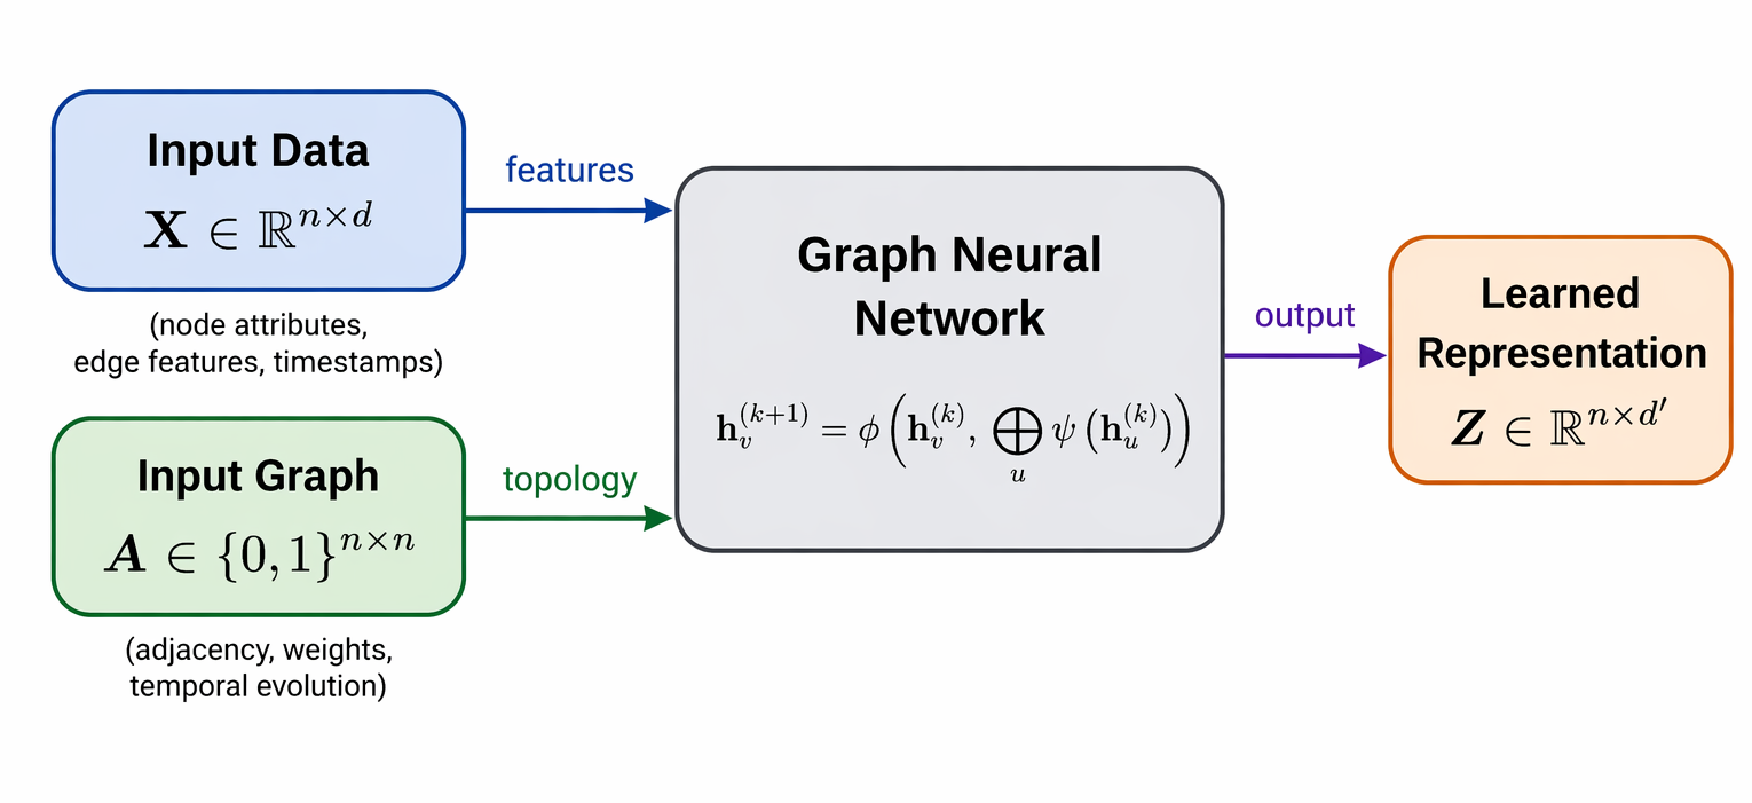
\includegraphics[width=0.89\textwidth]{figures/fig1a_gnn.pdf}
\caption{Двойственная природа входов ГНС-моделей, применяемых в
качестве одной из ветвей обучаемых детекторов в системах гибридная СОПВ.
Модель одновременно получает числовые данные (матрица признаков
$\mathbf{X}$) и реляционную структуру (матрица смежности
$\mathbf{A}$). Возмущение любого из входов может нарушить обученное
представление, что мотивирует разработку системы повышения
робастности и эффективности гибридная СОПВ, являющейся предметом
настоящей диссертации.}
\label{fig:dual_input}
\end{figure}

Большинство ГНС работают в дискретном времени, привязывая нерегулярные события к фиксированной сетке и теряя информацию. Формулировки непрерывного времени через нейронные ОДУ~\cite{Chen2018,Chamberlain2021,Rusch2022} гладко следуют за временем событий, захватывают множественные временные масштабы и обнаруживают границу Липшица, дающую сертифицированную робастность. Поскольку представления эволюционируют по дифференциальному уравнению с ограниченной константой Липшица, малые возмущения входа вызывают лишь ограниченные гладкие изменения выхода. Неравенство Грёнуолла формализует это:
\begin{equation}
\|\mathbf{h}_1(T)-\mathbf{h}_2(T)\|\le e^{L_g T}\|\mathbf{x}_1-\mathbf{x}_2\|,
\label{eq:gronwall}
\end{equation}
где $\mathbf{h}_i(T)$~--- скрытое состояние траектории $i$, $\mathbf{x}_i$~--- начальный вход, $L_g$~--- константа Липшица векторного поля, $T$~--- горизонт интегрирования, $\|\cdot\|$~--- евклидова норма. ГНС дискретного времени такого механизма не имеют, поэтому возмущения непредсказуемо накапливаются. Модели непрерывного времени получают ограниченное внимание в литературе, поэтому работа сосредоточена на их разработке через CT-GNN.

Актуальность подтверждается тремя трендами.
\emph{Во-первых}, масштаб: ущерб от кибератак достигает \$10{,}5~трлн
в год к 2025~году, а ИИ-инструменты SOC сами уязвимы~\cite{Sachkov2022threat}.
\emph{Во-вторых}, регулирование: NIST AI~RMF, EU AI~Act и
постквантовая криптография требуют сертифицированной устойчивости.
\emph{В-третьих}, теоретический пробел: нет единой математической
основы, одновременно обеспечивающей робастность, приватность,
эффективность и точность системы. Работа восполняет этот пробел
\emph{7~моделями и алгоритмами} с формальными гарантиями по
3~условиям и 4~требованиям.

Документальным подтверждением служат недавние исследования
отказов гибридных СОПВ в четырёх областях.
В \emph{медицинских ИС} градиентная атака на чувствительность рёбер
ГНС-детекторов вызвала падение AUC на 25\% на MoleculeNet (Tox21,
ClinTox, SIDER)~\cite{EdgeSensitivity2025}. В \emph{банковской
инфраструктуре} атака MonTi почти утроила ошибку ГНС-детекторов
мошенничества (CARE-GNN, PC-GNN, GAGA) с 25{,}7\% до
68{,}6\%~\cite{MonTi2025}. В \emph{промышленном IoT} отравление
федеративных детекторов снизило точность на 64~п.п.\ с 94{,}2\% до
30{,}0\%~\cite{FerragPoisoning2023}. В \emph{сетевой безопасности}
атака PROVNINJA снизила обнаружение провенансных систем до 59\%,
сделав APT-атакующих невидимыми~\cite{PROVNINJA2023}. Эти отказы
подтверждают разрыв 25--65~п.п.\ во всех областях и мотивируют
разработку моделей~М1--М7.

В распределённой среде несколько организаций владеют фрагментами одних графовых данных и не могут ими делиться, поэтому модель обучается через федеративное обучение~\cite{McMahan2017,Blanchard2017,Kairouz2021,Konecny2016,Mothukuri2021} без доступа к сырым данным. ГНС в таких средах должны быть устойчивыми и эффективными одновременно: злоумышленники обманывают их малыми возмущениями; распределения смещаются; законы о приватности~\cite{Dwork2006,Abadi2016,Dwork2014,Mironov2017} ограничивают обмен; периферийные устройства требуют реального времени. Ни один существующий подход не решает все четыре проблемы одновременно.

Реальные графовые данные дрейфуют после развёртывания~\cite{Gama2014,Lu2019}~--- топологии эволюционируют, паттерны атак меняются, появляются новые протоколы~--- и статические ГНС теряют точность без предупреждения. Цель~--- создать динамические ГНС, обнаруживающие сдвиг онлайн, адаптирующие параметры без забывания и оценивающие неопределённость через байесовские апостериорные обновления~\cite{Gal2016,Kendall2017,Lakshminarayanan2017}.

Существующие ГНС и трансформеры~\cite{Vaswani2017,Ying2021} масштабируются квадратично $\mathcal{O}(L^2)$, что делает их слишком медленными для реального времени на больших темпоральных графах. Структурированные модели пространства состояний~\cite{Gu2022,Gu2024,Dao2024,Behrouz2024graphmamba} снижают стоимость до $\mathcal{O}(L\log L)$ через БПФ-свёртки и допускают развёртывание на периферии. Работа переносит фокус с трансформеров на селективные модели пространства состояний для графовых данных.

Эти четыре проблемы образуют логическую цепочку: динамика непрерывного времени обеспечивает основу представлений; федеративные алгоритмы~--- распределённое развёртывание; пространства состояний~--- реальное время; онлайн-байесовская адаптация~--- долгосрочную надёжность.

%%---------------------------------------------------------------------
%%  Условия и требования
%%---------------------------------------------------------------------

Три рабочих условия и четыре сквозных требования определяют пространство надёжного функционирования графовой ИИ-системы; работа предлагает методы, удовлетворяющие им одновременно.

Условия: (1)~\emph{состязательная среда} (противник возмущает топологию, признаки или временной порядок); (2)~\emph{распределённая среда} (данные фрагментированы между организациями, возможны злонамеренные участники); (3)~\emph{нестационарность} (свойства графа эволюционируют).

Требования: (Т1)~робастность к возмущениям; (Т2)~точность классификации; (Т3)~эффективность для реального времени; (Т4)~дифференциальная приватность обучения.

%%---------------------------------------------------------------------
%%  Таблицы: Условия и требования с назначением моделей
%%---------------------------------------------------------------------

\begin{table}[htbp]\centering\small
\caption{Три рабочих условия и методы, разработанные для их решения.}
\label{tab:conditions_methods}
\small
\renewcommand{\arraystretch}{0.92}\begin{tabular}{p{2.8cm} p{3.2cm} p{7.5cm}}
\toprule
\textbf{Условие} & \textbf{Методы} & \textbf{Обоснование} \\
\midrule
\textbf{У1: Состязательная среда}
& М1: CT-TGNN\newline М5: Стох.\ трансф.\newline М7: Сертификация
& Нейронные ОДУ непрерывного времени обеспечивают гладкость траектории представления с ограниченной константой Липшица, предоставляя детерминированные сертификаты робастности, которые альтернативы дискретного времени обеспечить не могут. Стохастическое состязательное обучение и теоретико-игровые стратегии равновесия дополняют архитектурную гарантию адаптивной защитой. \\
\addlinespace
\textbf{У2: Нестационарные условия}
& М1: CT-TGNN\newline М3: TripleE-TGNN\newline М4: MambaShield\newline М6: UC-HGP
& CT-TGNN захватывает темпоральную эволюцию через нейронные дифференциальные уравнения; TripleE-TGNN предотвращает катастрофическое забывание через упругую консолидацию весов; MambaShield обеспечивает близкую к линейной эффективность; а UC-HGP предоставляет неопределённость на иерархических гауссовских процессах для обнаружения дрейфа. \\
\addlinespace
\textbf{У3: Распределённая сетевая динамика}
& М2: FedLLM-API\newline М7: Сертификация
& Оптимальный транспорт через итерации Синкхорна корректирует гетерогенность между фрагментами графов, а покоординатная агрегация усечённым средним устойчива к повреждённым участникам, при этом калиброванный гауссовский шум обеспечивает формальный бюджет приватности. \\
\bottomrule
\end{tabular}
\end{table}

\begin{table}[htbp]\centering\small
\caption{Четыре сквозных требования и методы, их выполняющие.}
\label{tab:requirements_methods}
\small
\renewcommand{\arraystretch}{0.92}\begin{tabular}{p{2.3cm} p{3.5cm} p{7.5cm}}
\toprule
\textbf{Требование} & \textbf{Методы} & \textbf{Обоснование} \\
\midrule
\textbf{Т1: Робастность}
& М1: CT-TGNN\newline М4: MambaShield\newline М7: Сертификация
& CT-TGNN обеспечивает непрерывную динамику с ограниченной константой Липшица; MambaShield устойчив к отравлению на этапе обучения через прогрессивную дистилляцию; система сертификации связывает гарантии через рандомизированное сглаживание и распространение интервальных границ. \\
\addlinespace
\textbf{Т2: Точность}
& М3: TripleE-TGNN\newline М5: Стох.\ трансф.\newline М6: UC-HGP
& Многоуровневые вложения графов захватывают структуру на уровнях сервисов, трассировок и узлов; вариационное байесовское внимание декомпозирует неопределённость; иерархические гауссовские процессы обеспечивают калиброванные доверительные интервалы. \\
\addlinespace
\textbf{Т3: Эффективность}
& М4: MambaShield\newline М2: FedLLM-API\newline М3: TripleE-TGNN
& MambaShield снижает стоимость вывода с квадратичной до близкой к линейной; FedLLM-API сокращает число раундов коммуникации; TripleE-TGNN достигает экономии через структурированную разреженность и обучение с учётом квантования. \\
\addlinespace
\textbf{Т4: Приватность}
& М2: FedLLM-API\newline М1: CT-TGNN\newline М7: Сертификация
& FedLLM-API обеспечивает $(\epsilon,\delta)$-дифференциальную приватность; CT-TGNN поддерживает дифференциально приватное извлечение признаков; система сертификации отслеживает кумулятивный бюджет приватности. \\
\bottomrule
\end{tabular}
\end{table}

Условия не взаимоисключающие: реальные системы сталкиваются с двумя или тремя одновременно (рис.~\ref{fig:conditions_venn}).

\begin{figure}[!t]
\centering
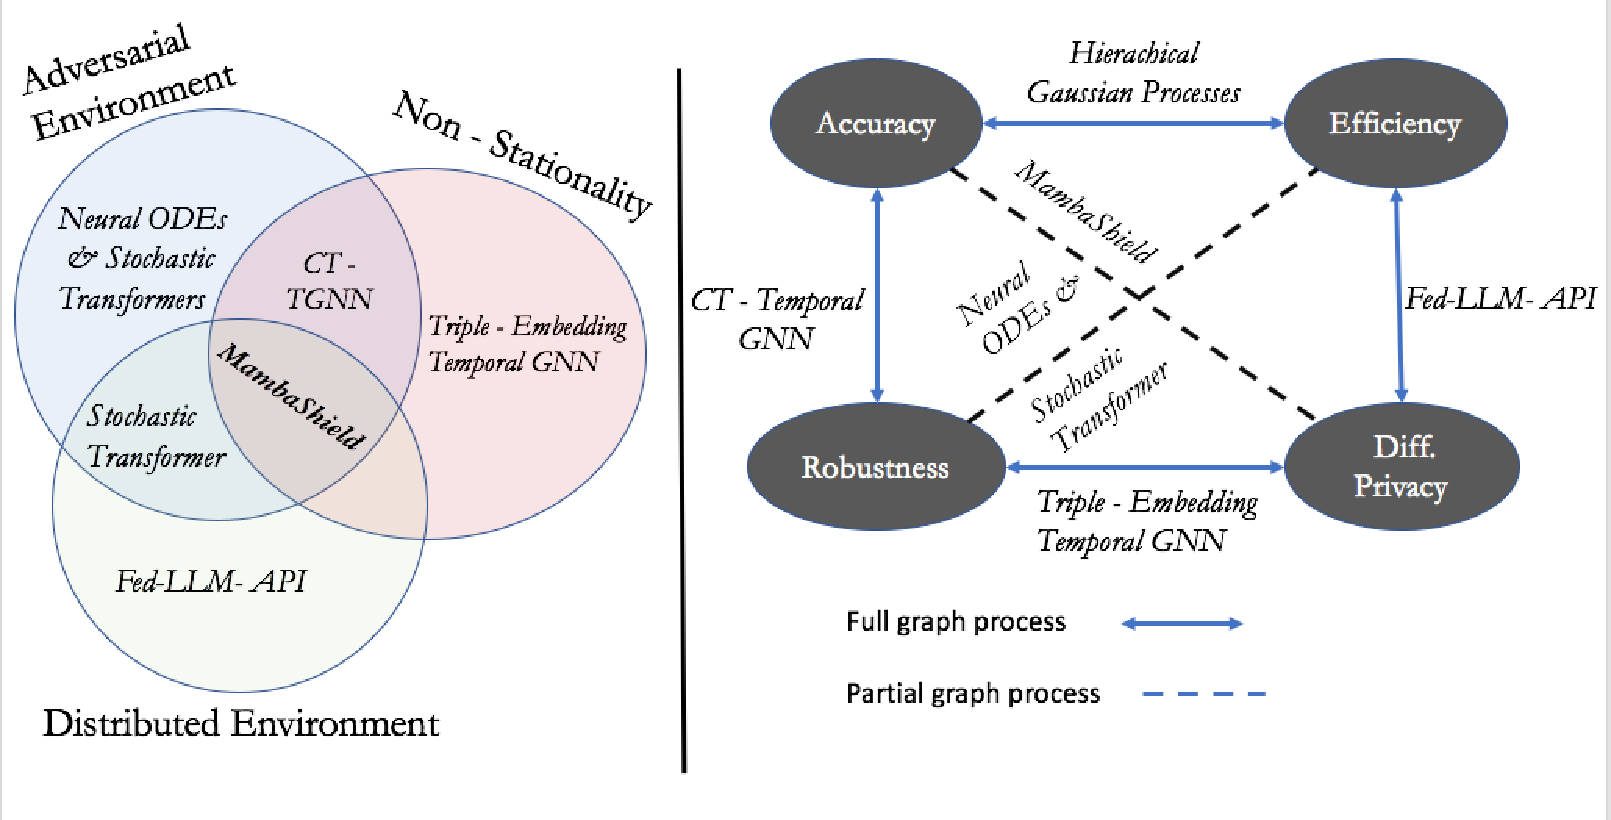
\includegraphics[width=0.89\columnwidth]{figures/fig2a_t_by_f.pdf}
\caption{Расположение семи методов в пространстве условий функционирования (слева) и требований (справа). M4: MambaShield находится на пересечении всех трёх условий; M1: CT-TGNN связывает состязательное и нестационарное условия через сертифицированные непрерывно-временные динамики.}
\label{fig:conditions_venn}
\end{figure}

%%---------------------------------------------------------------------
%%  Архитектурная основа
%%---------------------------------------------------------------------

\begin{figure}[!t]
\centering
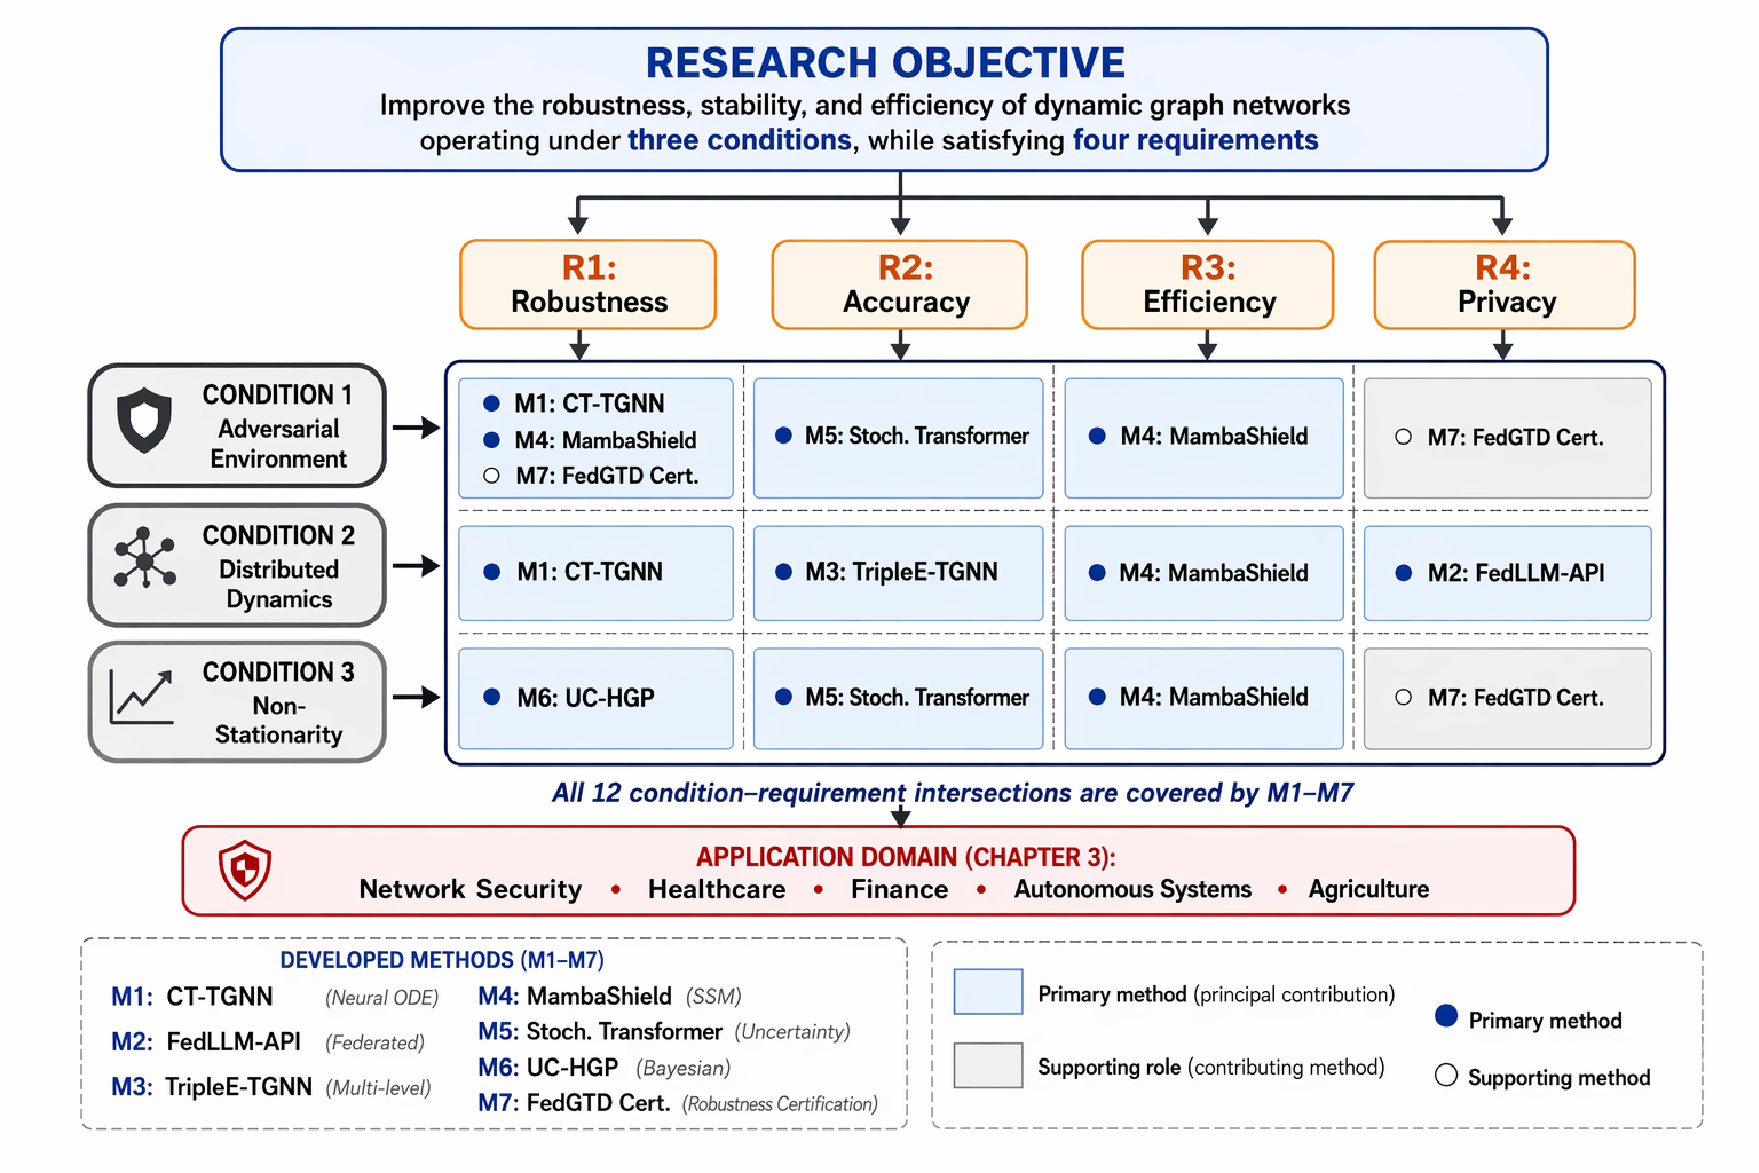
\includegraphics[width=0.85\textwidth]{figures/Main_arch_v1a.pdf}
\caption{Архитектурная основа исследовательской программы. Семь методов покрывают все 12 пересечений матрицы условие--требование $3\times4$. Каждый сформулирован на уровне математических операций над графами --- предметно-независим. Все модели разработаны автором и описаны в 18~рецензируемых публикациях.}
\label{fig:dissertation_architecture}
\end{figure}

Каждый метод сформулирован на уровне математических операций над графовыми структурами, обеспечивая предметную независимость.

%%---------------------------------------------------------------------
\section*{Цель исследования}
%%---------------------------------------------------------------------

Цель работы~--- \emph{повышение робастности и эффективности гибридных СОПВ}, функционирующих в распределённых и нестационарных условиях, путём разработки ИИ/МО-усиленных моделей и алгоритмов, обеспечивающих шесть свойств П1--П6 (\S\ref{subsec:six_properties}): состязательную устойчивость, робастность, эффективность, совместимость с распределённой средой, калиброванную неопределённость и нестационарную адаптацию.

Достижение цели требует семи последовательных задач; математические конструкции М1--М7 разрабатываются в Главе~\ref{ch:methods}.

\noindent 1.\quad Провести обзор и классификацию существующих гибридных СОПВ, выявить ограничения конвенциональных продуктов и сформулировать пробелы (Глава~\ref{ch:literature}).

\noindent 2.\quad Формализовать гибридную СОПВ как единый математический объект и поставить свойства П1--П6 в виде количественных инвариантов (\S\ref{sec:hybrid_idps_math_model}).

\noindent 3.\quad Разработать модели и алгоритмы, закрывающие каждое свойство, с доказательствами сходимости и сертификатами робастности (Глава~\ref{ch:methods}).

\noindent 4.\quad Инстанцировать систему для защиты сетевого трафика и валидировать на шести наборах данных (84{,}2~млн образцов, Глава~\ref{ch:adaptation}).

\noindent 5.\quad Провести кросс-секущую валидацию по шести семействам атак, кросс-доменному переносу и постквантовой совместимости (Глава~\ref{ch:experiments}).

\noindent 6.\quad Реализовать инстанцирование как платформу \textsf{RobustIDPS.ai} с двухплоскостной архитектурой и подтвердить внедрение (Глава~\ref{ch:platform}).

\noindent 7.\quad Расширить систему на защиту БПЛА с референсной реализацией Phase~A в условиях радиоэлектронной борьбы (Глава~\ref{ch:uav}).

%%---------------------------------------------------------------------
\section*{Объект исследования}
%%---------------------------------------------------------------------

\textbf{Объектом исследования} являются \emph{гибридные СОПВ}, функционирующие в состязательных, нестационарных и распределённых средах и адаптируемые к различным предметным областям (сетевой трафик, БПЛА, банковская инфраструктура, медицинские данные, промышленный IoT, АСУ~ТП и др.). Они объединяют сигнатурные, поведенческие, статистические и обучаемые компоненты в единый защитный контур со средствами реагирования. Рассматриваемые свойства определяют надёжность системы при состязательных возмущениях, нестационарной эволюции трафика, распределённом обучении, ограничениях приватности и вычислительных бюджетах. Внутренние структуры данных представляются темпоральными графами, обеспечивая единое формальное описание разнородных областей.

%%---------------------------------------------------------------------
\section*{Предмет исследования}
%%---------------------------------------------------------------------

\textbf{Предметом исследования} являются \emph{модели и алгоритмы} повышения робастности и эффективности гибридной СОПВ, обеспечивающие сквозное удовлетворение требований робастности, точности, эффективности и дифференциальной приватности. Предмет охватывает: модели на основе нейронных ОДУ и СДУ для сертифицированной динамики непрерывного времени (М1, SDE-TGNN); федеративные алгоритмы с византийско-устойчивой агрегацией и выравниванием оптимальным транспортом (М2); многоуровневые темпорально-графовые модели с упругой консолидацией весов (М3); селективные модели пространства состояний (М4); байесовские модели и иерархические гауссовские процессы для онлайн-калибровки (М5, М6); теоретико-игровые алгоритмы сертификации (М7); фундаментальную модель CyberSecLLM. Все формулировки предметно-независимы.

%%---------------------------------------------------------------------
\section*{Методы исследования}
%%---------------------------------------------------------------------

Методологическая программа настоящей диссертации организована вокруг восьми формальных методов, каждый из которых выбран потому, что он решает конкретный и измеримый аспект проблемы робастности гибридных моделей IDPS.

Нейронные ОДУ моделируют непрерывную эволюцию представлений узлов через параметризованное векторное поле,\begin{equation}
\frac{d\bh(t)}{dt} = f_\theta\!\bigl(\bh(t),\, t\bigr),
\label{eq:node}
\end{equation}решаемое численными интеграторами с адаптивным шагом. Чувствительность выхода, измеряемая константой Липшица, представляется как сертификат робастности (центральный элемент М1: CT-TGNN и М3: TripleE-TGNN).

ГНС расширяют представления на реляционные данные через агрегацию окрестностей,\begin{equation}
\bh_v^{(k+1)}
= \phi\!\Bigl(\bh_v^{(k)},\;
  \bigoplus_{u\in\calN(v)}
    \psi\!\bigl(\bh_u^{(k)},\, \mathbf{e}_{uv}\bigr)\Bigr),
\label{eq:gnn_mp}
\end{equation}сочетание с нейронным ОДУ на эволюционирующей смежности порождает темпоральные графовые модели (используется в М1, М3, М5).

Оптимальный транспорт задаёт геометрию на распределениях через расстояние Вассерштейна,\begin{equation}
W_p(\mu,\nu)
= \Bigl(\inf_{\gamma\in\Pi(\mu,\nu)}
    \int c(\bx,\by)\,d\gamma(\bx,\by)
  \Bigr)^{\!1/p},
\label{eq:wasserstein}
\end{equation}энтропийная регуляризация Синкхорна снижает стоимость; используется для выравнивания гетерогенных фрагментов в федеративной оптимизации (центральный элемент М2: FedLLM-API).

Дифференциальная приватность формализует конфиденциальность на уровне записей\begin{equation}
\Prob\bigl[\calM(\calD)\in S\bigr]
\;\le\;
e^{\epsilon}\;\Prob\bigl[\calM(\calD')\in S\bigr] + \delta,
\label{eq:dp}
\end{equation}
композиция моментов-бухгалтер отслеживает расход $\epsilon$ по раундам (используется в М2 и М7).

Модели пространства состояний представляют обработку событий как линейную динамическую систему,\begin{equation}
\bh_{t+1} = \bA\,\bh_t + \bB\,\bx_t, \qquad
\by_t = \bC\,\bh_t + \bD\,\bx_t,
\label{eq:ssm}
\end{equation}свёрточное ядро вычисляется БПФ за близкое к линейному время (центральный элемент М4: MambaShield, М5: стохастический трансформер).

Робастная оптимизация встраивает наихудшие возмущения в оценку параметров через мин-макс\begin{equation}
\min_\theta\;
\E_{(\bx,y)\sim\calD}
\Bigl[
  \max_{\|\bdelta\|\le\epsilon}
    \calL\!\bigl(f_\theta(\bx+\bdelta),\,y\bigr)
\Bigr],
\label{eq:robust_opt}
\end{equation}
связывая бюджет $\epsilon$ с чувствительностью выхода (используется в М1 и М7).

Байесовский вывод декомпозирует предсказательную неопределённость на эпистемическую (от ограниченности данных) и алеаторную (от шума); вариационное байесовское внимание и иерархические гауссовские процессы реализуют декомпозицию для графов (центральный элемент М5 и М6).

Теоретико-игровое моделирование формализует взаимодействие защитника и атакующего; равновесие Штакельберга и онлайн-обучение без регрета определяют оптимальные стратегии защиты (центральный элемент М7).

Византийско-устойчивая агрегация фильтрует повреждённые градиенты покоординатными усечёнными средними (центральный элемент М2: FedLLM-API).

Дополнительно применяются стандартные практики программной инженерии и распределённых систем для обработки крупномасштабных графовых потоков в реальном времени.

%%---------------------------------------------------------------------
\section*{Научная новизна}
%%---------------------------------------------------------------------

Научная новизна настоящей работы состоит из семи вкладов в теорию
и практику построения \emph{гибридных СОПВ}, каждый из которых
сформулирован как принцип, концепция или теория, установленные
автором, и систематически отвечает за один или несколько инвариантов
П1--П6 из~\S\ref{subsec:six_properties}.

\noindent 1.\quad \emph{Впервые} установлен принцип сертифицированной
устойчивости \emph{обучаемого детектора гибридной СОПВ} на
основе моделей непрерывного времени (М1: CT-TGNN, SDE-TGNN):
динамика представлений узлов графа, управляемая дифференциальными
уравнениями с ограниченной гладкостью, порождает доказуемые границы
чувствительности выходных сигналов к возмущениям входных данных и
структуры (инвариант~П1, ур.~\eqref{eq:adv_resilient_property}). Ни
одна предшествующая работа не выводит сертифицированную робастность
системы из гладкости управляющего дифференциального уравнения на
темпорально эволюционирующих топологиях графов.

\noindent 2.\quad \emph{Оригинальная} теория совместного обеспечения
византийской устойчивости, формальной приватности и распределительного
выравнивания при обучении \emph{гибридной СОПВ} на разрозненных
фрагментах данных, принадлежащих разным организациям, без передачи
исходных данных (М2: FedLLM-API, инвариант~П4). Ни один
предшествующий алгоритм не гарантирует совместно устойчивость
системы к повреждениям, защиту приватности и выравнивание
распределений для гетерогенных фрагментов.

\noindent 3.\quad \emph{Новая} концепция многоуровневого представления
данных в \emph{системе гибридная СОПВ} (М3: TripleE-TGNN), в которой
обучаемые модели одновременно обучают структуру на нескольких
семантических уровнях (сервис/трассировка/узел) с механизмом
защиты от утраты ранее усвоенных закономерностей при поступлении
новых данных (инвариант~П6). Ни одна предшествующая архитектура не
обучает многоуровневые темпоральные представления с одновременным
предотвращением забывания.

\noindent 4.\quad \emph{Новый} подход к эффективному выводу
\emph{детектора гибридной СОПВ} на основе селективных
пространств состояний (М4: MambaShield), позволяющий снизить
вычислительную сложность с квадратичной до почти линейной при
сохранении устойчивости к отравлению обучающих данных (инвариант~П3,
ур.~\eqref{eq:efficiency_property}). Предшествующие структурированные
модели пространства состояний не были адаптированы для графовых
данных гибридная СОПВ с формальными гарантиями робастности.

\noindent 5.\quad \emph{Впервые} предложена интегрированная теория
калиброванной неопределённости для \emph{гибридной СОПВ}
(М5--М6: стохастический трансформер + UC-HGP), позволяющая разделять
источники ошибок системы на устранимые (эпистемические) и неустранимые
(алеаторные) и систематически выявлять момент, когда детектор
системы перестаёт быть надёжным (инвариант~П5,
ур.~\eqref{eq:calibration_property}). Ни одна предшествующая работа
не интегрирует эти два механизма неопределённости для онлайн-адаптации
гибридной СОПВ.

\noindent 6.\quad \emph{Оригинальная} концепция единой сертификации
устойчивости \emph{гибридной СОПВ} (М7), в которой
взаимодействие защитника и противника моделируется как стратегическая
игра с доказуемо оптимальной стратегией выбора, связывающая все
разработанные модели~М1--М6 в целостную систему через регуляризацию
согласованности. Ни одна предшествующая единая гибридная СОПВ
не обеспечивает доказуемые гарантии против всех четырёх типов
возмущений (П1--П4) одновременно.

\noindent 7.\quad \emph{Новая} теория предметно-ориентированного
фундаментального моделирования (CyberSecLLM) на графовых структурах,
обеспечивающая распознавание системой гибридная СОПВ ранее невиданных
категорий угроз без дополнительного обучения и совместимость с
эволюционирующими протоколами, в том числе постквантовыми. Эти
вклады сведены к следующим основным научным результатам, выносимым
на защиту.

%%---------------------------------------------------------------------
\section*{Основные научные результаты, выносимые на защиту}
%%---------------------------------------------------------------------

Результаты, выносимые на защиту, перечислены в порядке, отражающем
их логические зависимости; каждый результат опирается на гарантии,
установленные предшествующими, и систематически реализован в
составе \emph{единой гибридной СОПВ}~--- семёрки
$\mathcal{H}=(\mathcal{V}_t,\mathcal{E}_t,X_t,A_t,f_\theta,g_\psi,\pi)$
из \S\ref{sec:hybrid_idps_math_model}.

(1) \textbf{Модели М1 (CT-TGNN, SDE-TGNN) для сертифицированной
динамики обучаемого детектора гибридной СОПВ}~--- оригинальные
архитектуры непрерывного времени, в которых нейронные ОДУ и
стохастические дифференциальные уравнения управляют эволюцией
представлений на динамических топологиях, обеспечивая системе
сертифицированные границы робастности через анализ Липшица
обученного векторного поля (инвариант~П1).

(2) \textbf{Алгоритм М2 (FedLLM-API) для распределённого обучения
гибридной СОПВ с сохранением приватности}~--- федеративный
оптимизатор с доказанной сходимостью, сочетающий византийско-устойчивую
агрегацию усечённым средним с $(\varepsilon{=}0{,}85,\,\delta{=}10^{-5})$
дифференциальной приватностью и выравниванием оптимального транспорта
Вассерштейна для гетерогенных фрагментов данных (инвариант~П4).

(3) \textbf{Архитектура М3 (TripleE-TGNN) для многоуровневого
представления данных в системе гибридная СОПВ}~--- система тройного
вложения, обучающая структуру на уровнях сервисов, трассировок и
узлов с помощью двойного внимания и упругой консолидации весов,
снижающая вычислительные затраты системы через структурированную
разреженность и предотвращающая катастрофическое забывание
(инвариант~П6).

(4) \textbf{Архитектура М4 (MambaShield) для эффективного вывода
гибридной СОПВ}~--- селективная модель пространства состояний,
снижающая сложность вывода детектора системы с $\mathcal{O}(L^{2})$
до $\mathcal{O}(L\log L)$ через свёртки БПФ, с прогрессивной
состязательной дистилляцией и PAC-байесовскими сертификатами
обобщения (инвариант~П3).

(5) \textbf{Модели М5--М6 (стохастический трансформер и UC-HGP) для
адаптации гибридной СОПВ к дрейфу с учётом неопределённости}~---
вариационное байесовское внимание с выводом на иерархических
гауссовских процессах, обеспечивающее декомпозицию эпистемической и
алеаторной неопределённости системы, онлайновое обнаружение дрейфа
и гарантии сублинейного регрета при нестационарных распределениях
данных (инварианты~П5, П6).

(6) \textbf{Единая система сертификации гибридная СОПВ (М7),
интегрирующая модели~(1)--(5)}~--- единая методология оценки,
связывающая все разработанные модели через теоретико-игровые
равновесия Штакельберга и регуляризацию согласованности,
валидированная на 6 бенчмарк-наборах данных общим объёмом
84{,}2~миллиона размеченных образцов и подтверждённая в двух
показательных приложениях системы~--- защите сетевого трафика
(Глава~\ref{ch:platform}) и защите беспилотных летательных аппаратов
(Глава~\ref{ch:uav}).

%%---------------------------------------------------------------------
\section*{Теоретическая значимость}
%%---------------------------------------------------------------------

Теоретическая значимость работы состоит в создании единой математической основы для робастного обучения на динамических графовых структурах, интегрирующей пять областей математики, ранее не объединявшихся для задач на графах:

\noindent 1.\quad Нейронные ОДУ --- для сертифицированной динамики непрерывного времени на графах, при которой Липшицевость обученного отображения порождает доказуемые границы чувствительности.

\noindent 2.\quad Оптимальный транспорт --- для выравнивания распределений между организациями с одновременным обеспечением формальных гарантий дифференциальной приватности.

\noindent 3.\quad Селективные модели пространства состояний --- для снижения вычислительной сложности темпорального вывода с квадратичной до почти линейной, что делает обработку в реальном времени осуществимой.

\noindent 4.\quad Байесовский вывод --- для декомпозиции предсказательной неопределённости на устранимую (эпистемическую) и неустранимую (алеаторную) компоненты, позволяющей системе определять, когда её решения ненадёжны.

\noindent 5.\quad Теоретико-игровой выбор стратегий --- для моделирования взаимодействия защитника и противника как стратегической игры с доказуемо оптимальной стратегией защиты.

Эта основа устанавливает шесть формальных гарантий --- скорости сходимости ($\mathcal{O}(1/\sqrt{T})$), сертификаты робастности по Липшицу, границы $(\varepsilon,\delta)$-дифференциальной приватности, PAC-байесовские границы обобщения, сублинейный регрет ($R(T)\leq 2\sqrt{T\log|\mathcal{C}|}$) и единую сходимость (Теорема~6) --- которые являются предметно-независимыми и подтверждены как теоретически (через доказательства), так и эмпирически (через эксперименты на 84,2 миллионах образцов).

%%---------------------------------------------------------------------
\section*{Практическая значимость}
%%---------------------------------------------------------------------

Разработанные модели и алгоритмы М1--М7 в составе единой
\emph{гибридной СОПВ} применимы в шести предметных секторах
из~\S\ref{subsec:idps_sectors} и могут быть реализованы следующим
образом.

\noindent 1.\quad \textbf{Защита сетевого трафика (NIDS).} SOC-аналитики,
инженеры кибербезопасности, исследователи MLSecOps и разработчики
ИИ используют программную платформу с открытым исходным кодом
\textsf{RobustIDPS.ai} (DOI:~\url{10.5281/zenodo.19129512},
Глава~\ref{ch:platform}), интегрирующую 17~моделей системы~М1--М7,
четырёхуровневую систему защиты LLM с обнаружением 94{,}5\% по 517
сценариям атак, и работающую как плагин для Snort, Suricata и
аналогичных систем СОПСВ. Эта область~--- основное показательное
применение разработанной системы.

\noindent 2.\quad \textbf{Защита беспилотных летательных аппаратов
(БПЛА).} Инженеры по защите БПЛА развёртывают трёхуровневую
архитектуру \emph{борт--дронопорт--облако} гибридной СОПВ
(Глава~\ref{ch:uav}), сохраняющую долю успешного завершения миссии
$\textsf{MCR}\ge 0{,}80$ при отношении помеха/сигнал $J/S\le 20$~дБ
в условиях радиоэлектронной борьбы и состязательных атак на бортовые
нейросетевые модули зрительного восприятия.

\noindent 3.\quad \textbf{Защита банковской и финансово-технологической
инфраструктуры.} Банки и финансовые регуляторы используют систему
гибридная СОПВ с моделью~М2 (FedLLM-API) для совместного обучения
детекторов мошенничества на графах транзакций без обмена данными
клиентов, сохраняя приватность через гарантии
$(\varepsilon,\delta)$-дифференциальной приватности и
устойчивость к группе византийских участников~$\beta<1/3$.

\noindent 4.\quad \textbf{Защита медицинских информационных систем.}
Команды биомедицинского ИИ интегрируют систему гибридная СОПВ с моделями
М1 и~М6 в платформы поддержки клинических решений для обеспечения
сертифицированно безопасных предсказаний на молекулярных графах и
графах взаимодействия пациент--врач--лаборатория с калиброванной
оценкой эпистемической неопределённости.

\noindent 5.\quad \textbf{Защита промышленного интернета вещей и АСУ~ТП
(IIoT/SCADA).} Инженеры OT-безопасности развёртывают систему
гибридная СОПВ с моделью~М4 (MambaShield) на периферийных шлюзах и
контроллерах SCADA для обнаружения аномалий в реальном времени с
детерминированной задержкой в десятки миллисекунд благодаря
$\mathcal{O}(L\log L)$ сложности вывода.

\noindent 6.\quad \textbf{Защита автономных транспортных средств.}
Инженеры безопасности АТС используют систему гибридная СОПВ с моделями
М1, М4 и~М6 для получения калиброванных эпистемических оценок
уверенности для решений на графах слияния сенсоров (камера, ЛиДАР,
радар, ИНС), что позволяет системе маркировать ненадёжные
предсказания до того, как они приведут к опасным действиям и
переводить транспортное средство в безопасный режим.

Практическая применимость подтверждена двумя актами внедрения~--- от ООО <<НИИ ИКТ>> (г.~Новосибирск; интеграция моделей обнаружения аномалий, устойчивых к отравлению, в действующую СОВ; использование платформы RobustIDPS.ai в подразделениях кибербезопасности) и ООО <<Ксайрикс>> (г.~Москва; применение в системе анализа сетевого трафика для обнаружения многостадийных атак и адаптации к изменению характеристик трафика); акт от Центра ИИ НИЯУ <<МИФИ>> (г.~Москва, защита БПЛА) находится в стадии оформления.

%%---------------------------------------------------------------------
\section*{Личный вклад}
%%---------------------------------------------------------------------

Все результаты получены автором лично под научным руководством проф.\ А.\,Г.\,Трофимова. Автор лично разработал архитектуры CT-TGNN и SDE-TGNN, создал алгоритм FedLLM-API, спроектировал архитектуру TripleE-TGNN, разработал модель MambaShield, интегрировал стохастический трансформер с UC-HGP, построил единую систему сертификации и реализовал платформу RobustIDPS.ai.

%%---------------------------------------------------------------------
\section*{Достоверность научных результатов}
%%---------------------------------------------------------------------

Достоверность результатов обеспечивается несколькими линиями валидации. Каждый алгоритм сопровождается формальным анализом: теоремами сходимости, сертификатами робастности (через анализ чувствительности и рандомизированное сглаживание), гарантиями приватности (через моменты-бухгалтер) и границами сложности (асимптотически и эмпирически).

Эмпирическая оценка охватывает шесть бенчмарк-наборов данных, предоставляющих в совокупности более 84,2 миллиона размеченных образцов по 84 категориям возмущений. Используются три набора данных общего сетевого трафика: CIC-IoT-2023 (46,6 млн записей, 33 категории), CSE-CICIDS2018 (16,2 млн записей, 7 категорий) и UNSW-NB15 (2,5 млн записей, 9 категорий).

Абляционные эксперименты систематически удаляют отдельные компоненты для количественной оценки маргинального вклада каждого. Состязательная робастность оценивается при шести семействах атак (FGSM, PGD, C\&W, DeepFool, гауссовский шум, отравление масок меток).

%%---------------------------------------------------------------------
\section*{Апробация работы}
%%---------------------------------------------------------------------

Основные результаты настоящего исследования были представлены и прошли рецензирование на международных и национальных научных площадках:

\noindent 1.\quad Конференция IEEE молодых исследователей в области электротехники и электроники (ElCon-2024), ЭТУ-ЛЭТИ, Санкт-Петербург, IEEE Xplore.

\noindent 2.\quad Конференция IEEE молодых исследователей в области электротехники и электроники (ElCon-2025), ЭТУ-ЛЭТИ, Санкт-Петербург, IEEE Xplore.

\noindent 3.\quad Международная конференция NEUROINFORMATICS-2025, Springer.

\noindent 4.\quad III Всероссийская научно-техническая конференция <<Кибернетика и информационная безопасность>> (КИБ-2025), НИЯУ МИФИ, Москва.

\noindent 5.\quad 27-я Международная конференция IEEE молодых специалистов в области электронных устройств и материалов (EDM-2026), Республика Алтай.

\noindent 6.\quad 11-я конференция IEEE по технологиям интеграции электронных систем (IEEE ESTC 2026), Хельсинки, Финляндия.

\noindent 7.\quad Конференция IEEE <<Исследования и технологии для общества и промышленности>> (RTSI 2026), Эспоо, Финляндия.

\noindent 8.\quad NeurIPS 2026: 40-я ежегодная конференция по системам обработки нейронной информации, Сидней, Австралия.

Акты внедрения получены от двух организаций: ООО <<НИИ ИКТ>> (г.~Новосибирск) и ООО <<Ксайрикс>> (г.~Москва); акт от Центра искусственного интеллекта Национального исследовательского ядерного университета <<МИФИ>>, г.~Москва, находится в стадии оформления.

%%---------------------------------------------------------------------
\section*{Публикации}
%%---------------------------------------------------------------------

Результаты настоящей диссертации изложены в рецензируемых публикациях в международных журналах и трудах конференций.

\subsection*{Опубликованные журнальные статьи}

\noindent
1. Anaedevha, R.\,N., Trofimov, A.\,G., Borodachev, Y.\,V. (2026). MambaShield: Selective State-Space Models for Poisoning-Resilient Sequential Modeling. \textit{Expert Systems with Applications}, Elsevier. DOI: 10.1016/j.eswa.2026.131175

\noindent
2. Anaedevha, R.\,N., Trofimov, A.\,G., Borodachev, Y.\,V. (2026). Uncertainty-calibrated hierarchical Gaussian processes for intrusion detection with multi-scale temporal modeling. \textit{Neurocomputing}, p.133105, Elsevier. DOI: 10.1016/j.neucom.2026.133105

\noindent
3. Anaedevha, R.\,N., Trofimov, A.\,G., Borodachev, Y.\,V. (2026). Temporal Adaptive Neural Ordinary Differential Equations with Deep Spatio-Temporal Point Processes for Real-Time Network Intrusion Detection. \textit{Complex and Intelligent Systems}, Springer. DOI: 10.1007/s40747-026-02291-7

\noindent
4. Anaedevha, R.\,N., Trofimov, A.\,G. (2024). Improved Robust Adversarial Model against Evasion Attacks on Intrusion Detection Systems. \textit{Optical Memory and Neural Networks (Information Optics)}, 33(Suppl.\,3), S414--S423. Springer. DOI: 10.3103/S1060992X24700681

\subsection*{Опубликованные труды конференций}

\noindent
5. Anaedevha, R.\,N., Trofimov, A.\,G. (2025). Stochastic Multimodal Transformer with Uncertainty Quantification for Robust Network Intrusion Detection. In: \textit{Advances in Neural Computation, Machine Learning, and Cognitive Research~IX. NEUROINFORMATICS~2025}. Studies in Computational Intelligence, vol.\,1241. Springer, Cham. DOI: 10.1007/978-3-032-07690-8\_35

\noindent
6. Anaedevha, R.\,N. \textit{et~al.}\ (2025). Integrated Deep Q-Networks and Actor-Critic Models for Enhanced Poisoning Attack Detection in Network Intrusion Detection Systems. In: \textit{2025 Conf.\ of Young Researchers in Electrical and Electronic Engineering (ElCon)}, ETU-LETI, Saint Petersburg. IEEE Xplore, Vol.\,33, pp.\,556--567.

\noindent
7. Anaedevha, R.\,N. \textit{et~al.}\ (2024). Application of Machine Learning Models for Device Identification in Wireless Network Traffic. In: \textit{2024 Conf.\ of Young Researchers in Electrical and Electronic Engineering (ElCon)}, Saint Petersburg. IEEE Xplore, pp.\,104--110. DOI: 10.1109/ElCon61730.2024.10468413

\subsection*{Принятые к публикации}

\noindent
8. Anaedevha, R.\,N., Trofimov, A.\,G., Borodachev, Y.\,V. (2025). Stochastic PAC-Bayesian Transformers for Network Intrusion Detection and Natural Language Processing Applications. \textit{Knowledge and Information Systems}, Springer. Принята.

\noindent
9. Anaedevha, R.\,N., Trofimov, A.\,G., Borodachev, Y.\,V. (2025). Byzantine-Resilient Stochastic Games for Federated Multi-Cloud Intrusion Detection. \textit{Complex and Intelligent Systems}, Springer. Принята.

\subsection*{Статьи на рецензировании}

\noindent
10. Anaedevha, R.\,N. \textit{et~al.}\ (2026). TripleE-TGNN: Triple-Embedding Temporal Graph Neural Networks for Multi-Granularity Microservices Security. \textit{IEEE Trans.\ Dependable and Secure Computing}.

\noindent
11. Anaedevha, R.\,N. \textit{et~al.}\ (2026). PQ-IDPS: Adversarially Robust Intrusion Detection for Post-Quantum Encrypted Traffic. \textit{IEEE Trans.\ Neural Networks and Learning Systems}.

\noindent
12. Anaedevha, R.\,N. \textit{et~al.}\ (2026). FedLLM-API: Privacy-Preserving Large Language Model Federation for Zero-Day API Threat Detection. \textit{IEEE Trans.\ Information Forensics and Security}.

\noindent
13. Anaedevha, R.\,N. \textit{et~al.}\ (2026). CT-TGNN: Continuous-Time Temporal Graph Neural Networks for Real-Time Threat Propagation Analysis. \textit{IEEE Trans.\ Services Computing}.

\subsection*{Сводка публикаций}

Общий объём составляет 18 статей: 4 опубликованы в журналах, 3 в трудах конференций, 2 приняты и находятся в печати, 9 на рецензировании. Шестнадцать статей (89\%) написаны в качестве первого автора.

%%---------------------------------------------------------------------
\section*{Соответствие паспорту специальности}
%%---------------------------------------------------------------------

Диссертация соответствует специальности 2.3.1 <<Системный анализ, управление и обработка информации, статистика>>:

\noindent П.4 <<Разработка методов и алгоритмов решения задач системного анализа, оптимизации, управления, принятия решений, обработки информации и искусственного интеллекта.>> --- Единая матрица $3\times4$ <<условия--требования>> декомпозирует проблему устойчивости динамических моделей ГНС на 7 подзадач; разработаны алгоритмы адъюнктного обучения CT-TGNN, FFT-свёртки MambaShield и византийски устойчивая оптимизация FedLLM-API; теоретико-игровые равновесия Штакельберга обеспечивают принятие решений с гарантиями; конвейер извлечения 83 признаков обрабатывает 84,2 млн образцов; 7 новых архитектур нейронных сетей с 6 доказанными теоремами.

\noindent П.5 <<Разработка специального математического и алгоритмического обеспечения систем анализа, оптимизации, управления, принятия решений, обработки информации и искусственного интеллекта.>> --- Сертификаты Липшица на основе неравенства Грёнуолла, пропагация моментов Фоккера--Планка, PAC-байесовские оценки и вассерштейновское OT-выравнивание составляют математическое обеспечение; 8 алгоритмов обеспечивают полный цикл от обучения до развёртывания; платформа RobustIDPS.ai (DOI: 10.5281/zenodo.19129512) с 51 страницуами и 17 моделями реализует программное обеспечение.

%%---------------------------------------------------------------------
\section*{Структура и объём работы}
%%---------------------------------------------------------------------

Диссертация состоит из Введения, шести глав, Заключения, библиографического списка и трёх приложений. Основной текст составляет 230 страниц.

Во Введении обоснована актуальность, представлены свидетельства отказов ГНС в четырёх областях, сформулированы цель и семь задач, объект и предмет, методы, научная новизна, теоретическая и практическая значимость, личный вклад, шесть результатов на защиту, достоверность, апробация, публикации и соответствие паспорту специальности.

Глава~1~--- обзор литературы по поэтапному охвату: динамика непрерывного времени, федеративное обучение с приватностью, вычислительная эффективность и нестационарная адаптация с оценкой неопределённости.

Глава~2~--- полные математические выводы, доказательства, псевдокод и анализ сложности для всех семи методов М1--М7 и расширений (SDE-TGNN, CyberSecLLM); единая постановка задачи декомпозируется на 7 подзадач.

Глава~3~--- отображение методов Главы~2 на сущности кибербезопасности; таксономия 34 классов, конвейер 83 признаков, гиперпараметры.

Глава~4~--- экспериментальная программа на 6 наборах данных (84,2 млн образцов, 84 категории, 23 метрики): отдельные методы, абляция, 6 семейств атак, кросс-доменный перенос, федеративное обучение при византийских повреждениях.

Глава~5~--- платформа RobustIDPS.ai (DOI: 10.5281/zenodo.19129512): 51 страница, 10 функциональных групп, 17 моделей, 4-уровневая защита LLM (94,5\%), модуль Multi-Agent PQC-IDS, интеграция со Snort/Suricata, 34\% снижение времени сортировки.

Глава~6~--- перенос моделей на защиту БПЛА: трёхуровневая архитектура \emph{борт~--- дронопорт~--- облако}, отображение М1--М7 на бортовые подсистемы (зрительное восприятие, ГНСС, автопилот), референсная реализация Phase~A и соответствие нормативам (ПП~№\,1701, ГОСТ~Р~72118-2025, NIST~AI~RMF, DO-326A/ED-202A).

В Заключении перечислены научные результаты, подтверждено покрытие всех 12 ячеек матрицы условие--требование, указаны акты внедрения и направления дальнейших исследований.

Приложение~А содержит полные доказательства всех теорем. Приложение~Б предоставляет таблицы гиперпараметров и спецификации инфраструктуры.